\documentclass[a4paper,12pt]{book}

\usepackage[utf8]{inputenc}
\usepackage[hidelinks,bookmarks=true]{hyperref}
\usepackage[numbered]{bookmark}
\usepackage{graphicx}

\graphicspath{ {./pictures/} }

\title{
The AGE Framework
\linebreak
\linebreak
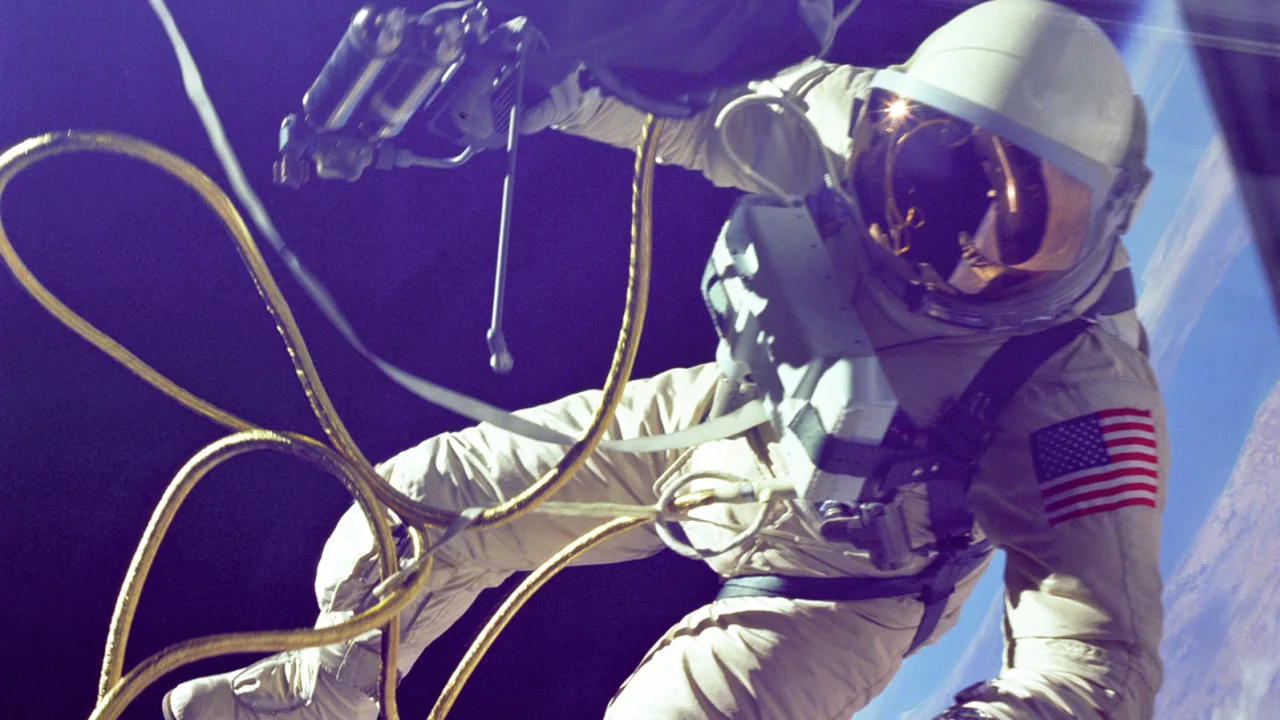
\includegraphics[width=8cm]{spacewalk.png}
}
\author{Philip Reichel}
\date{\today}

\begin{document}

\maketitle
\tableofcontents

\part{Concept}
This part presents the concept behind the framework and leads through the entire process from the initial vision to the final system requirements.
\begin{enumerate}
\item Design
\item Stakeholder
\end{enumerate}


\chapter{Introduction}
TBD

\section{Overview}
TBD

\section{Purpose}
TBD

\section{Goals}
TBD

\chapter{Stakeholders}
TBD

\section{Introduction}
TBD

\section{Purchasers}
TBD

\section{End Users}
TBD

\section{Developers}
TBD

\section{Operators}
TBD

\chapter{Use Cases}
TBD

\chapter{Stakeholder Needs}
TBD

\chapter{Requirements}
TBD

\section{Functional Requirements}
TBD

\section{Non Functional Requirements}
TBD

\subsection{Robustness}
TBD

\subsection{Reliability}
TBD

\subsection{Performance}
TBD

\subsection{Persistence}
TBD

\part{Design}
TBD

\part{Implementation}
TBD

\part{Testing}
TBD

\chapter{Resume}
TBD

\end{document}
